\documentclass{beamer}
\usepackage[utf8]{inputenc}
\usepackage[ngerman]{babel}
\usepackage{graphicx}
\usepackage{hyperref}

\title{Two-factor LUKS Decryption using YubiKey}
\author{Sree Harsha Totakura \\ {\footnotesize sreeharsha@totakura.in}}

\begin{document}
\begin{frame}
  \maketitle
\end{frame}

\begin{frame}
  \frametitle{About me}
  I~\ldots{}
  \begin{enumerate}
  \item use Full Disk Encryption with LUKS, always.
  \item paranoid about entering passwords, especially for FDE.
  \item Wish for a two-factor decryption for LUKS.
  \end{enumerate}
\end{frame}

\begin{frame}
  \frametitle{Two-Factor Decryption; How?}
  \begin{enumerate}
  \item Use a keyfile from a USB media to decrypt LUKS; USB media needs a
    password to unlock.
  \item Use a PGP smartcard to decrypt a keyfile; smartcard needs a PIN
  \item Use a \alert{YubiKey}
  \end{enumerate}
\end{frame}

\begin{frame}
  \frametitle{Yubikey}
  A USB device used to Authentication which generates OTPs. It \ldots{}
  \begin{enumerate}
  \item can store RSA keys
  \item generates OTP tokens using these keys
  \item can also do challenge response with these keys
  \item keys are only written, but never read. (really? Hmm, need to check on
    that.)
  \end{enumerate}
\end{frame}

\begin{frame}
  \frametitle{ykluks}
  \begin{center}
    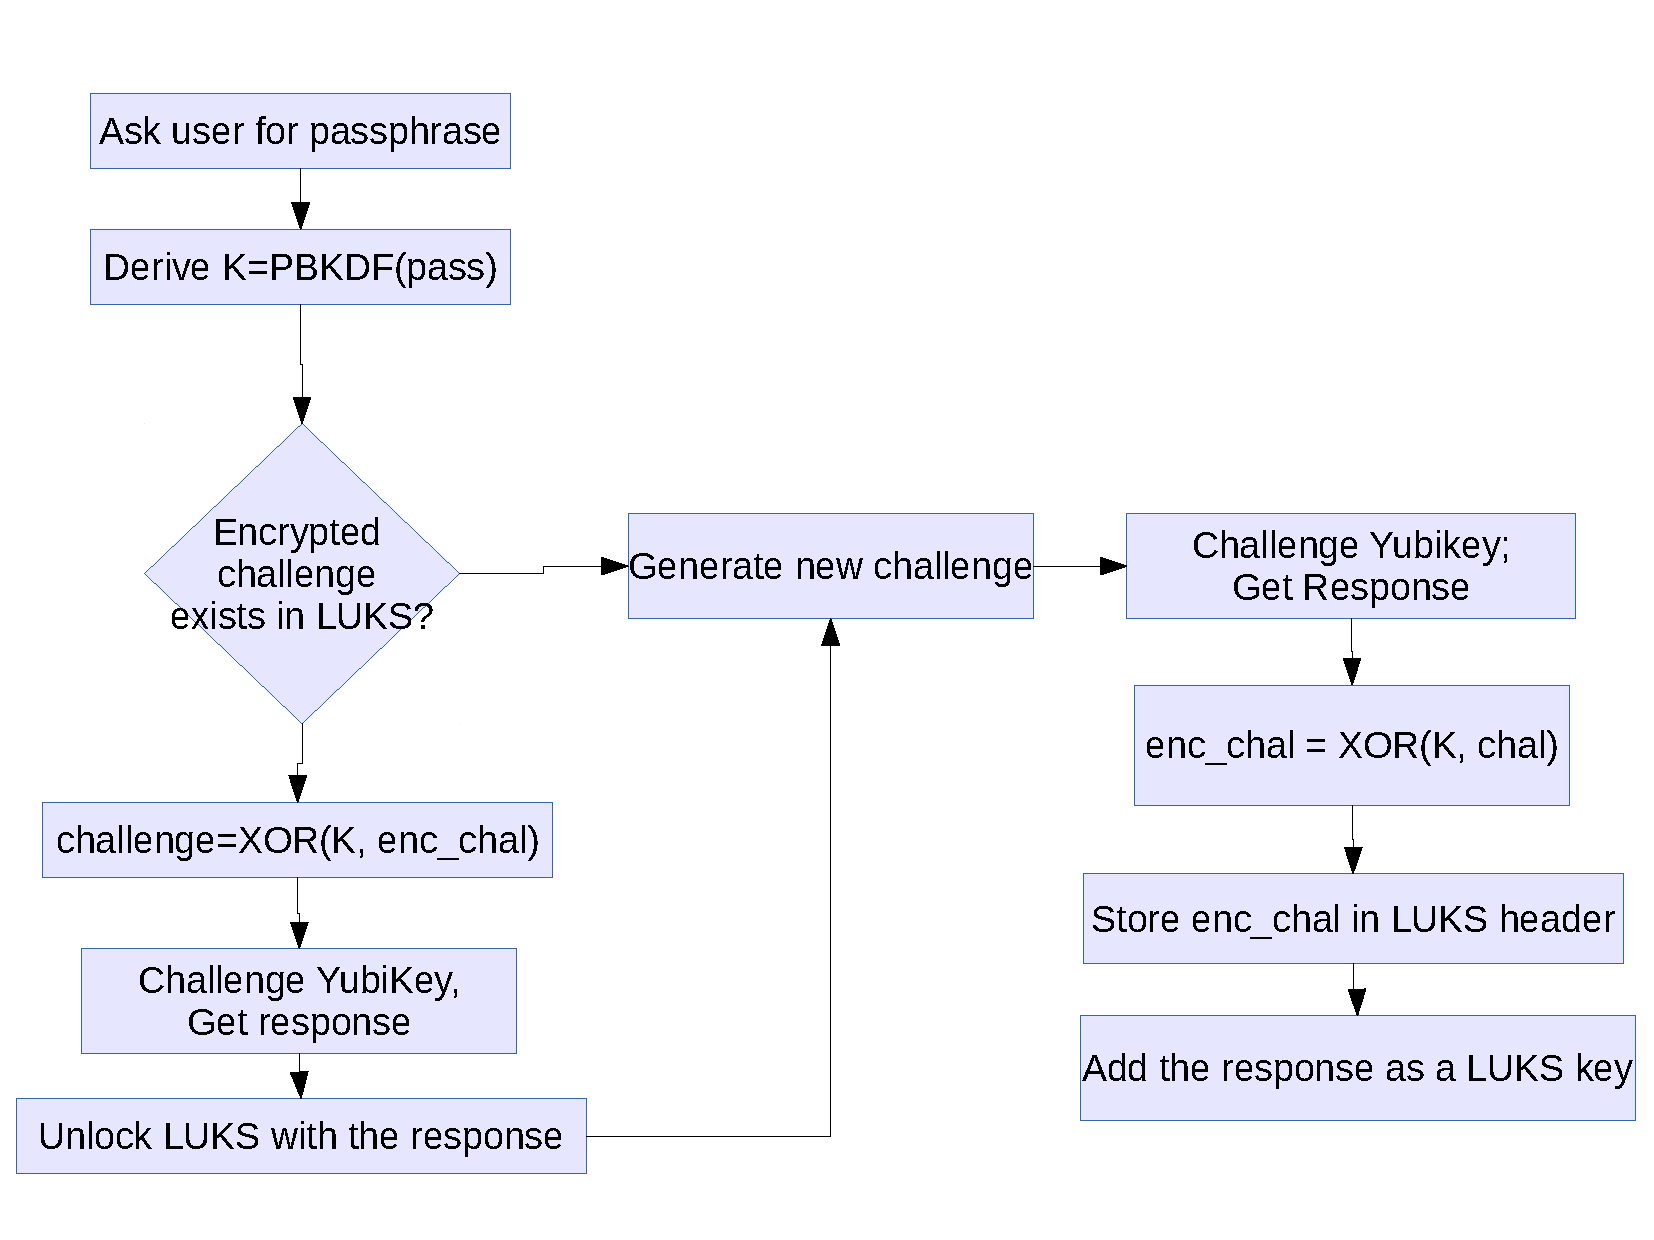
\includegraphics[width=\textwidth]{flowchart}
  \end{center}
\end{frame}

\begin{frame}
  \frametitle{Dirty bits}
  \begin{center}
    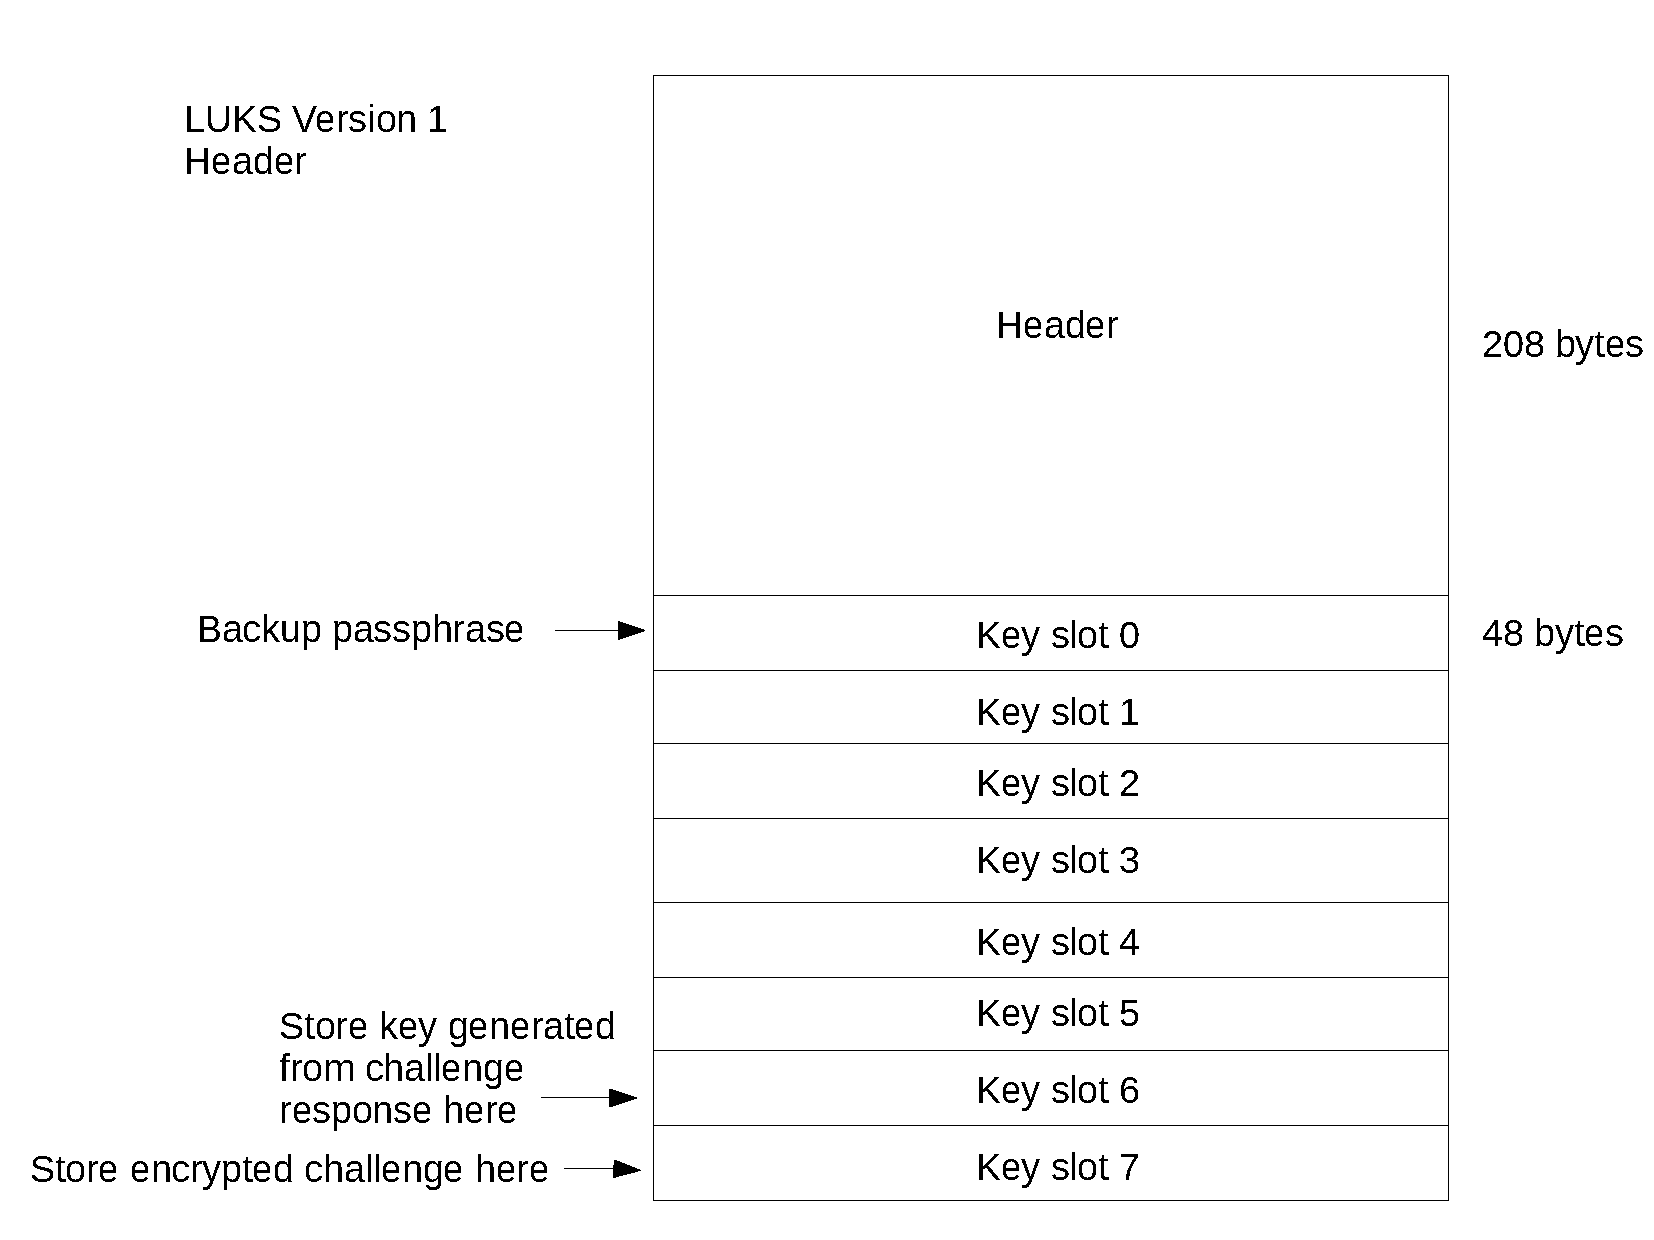
\includegraphics[width=\textwidth]{luks_header}
  \end{center}
\end{frame}

\begin{frame}
  \frametitle{Statutory Warning}
  \begin{center}
    Backup your LUKS header before using this.
  \end{center}
\end{frame}

\begin{frame}
  \frametitle{References}
  \begin{enumerate}
  \item \url{https://github.com/lfasnacht/ykluks}
  \item \url{https://github.com/totakura/ykluks} (with 2 factor auth; not merged
    into 1 yet)
  \item \url{https://github.com/cornelinux/yubikey-luks/blob/master/key-script}
  \end{enumerate}
\end{frame}

\begin{frame}
  \begin{center}
    Thank you
  \end{center}
\end{frame}

\end{document}
%%% Local Variables:
%%% mode: latex
%%% TeX-master: t
%%% End:
